\section{Test environment}\label{sec:testenvironment}
This chapter of the report describes the setup of the testing environment in which not only the tools during the research were tested, but also was used to test the System Readiness Inspector itself.
\\\\
A virtual network was set up on the Microsoft Azure Cloud as a test environment. The test network was set up in the cloud so that the development team can access the network regardless of its location. The test network consists of a Windows server and two Windows clients. Active Directory service was configured on the server to manage the client computer and to have the possibilities to create group policies. Group policies are used in almost every corporate environment to build rule sets for configurations. These configurations are a core element to check the readiness of a system. The following operating systems were installed in this test network: \\
\\
\textbf{Server:}
\begin{itemize}
    \item Windows Server 2016
\end{itemize}
\textbf{Clients:}
\begin{itemize}
    \item Windows 10 Pro, Version 1709
\end{itemize}
\ \\
The network is structured as followed:\\
\begin{figure}[H]
    \centering
    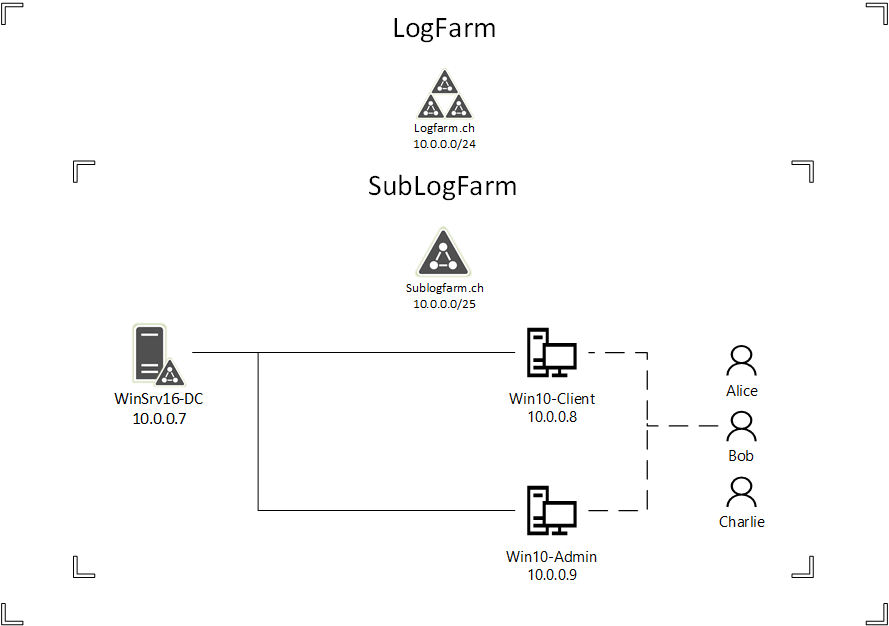
\includegraphics[width=0.9\linewidth]{assets/test-environment/testnetwork.png}
    \caption{Test Environment}
\end{figure}

\clearpage

\subsection{User}
Three users were configured for the logfarm-network:
\begin{table}[H]
    \centering
    \begin{tabular}{p{4cm} p{8cm}} \hline
        \textbf{Name} & \textbf{Privileges}  \\ \hline
        alice & Domain administrator  \\ \hline
        bob & User  \\ \hline
        charlie & User  \\ \hline
    \end{tabular}
    \caption{Test Environment User}
\end{table}

\subsection{Difficulties}
Various difficulties occurred which are presented in this subsection.
\paragraph{Connect to the virtuel machines via Remote Desktop Protocol (RDP)} \ \\
After setting up the virtual machines on Azure, the developers tried to connect to the devices via the Remote Desktop Protocol but failed. First, the developers suspected the issue was the incoming port rules, so the machines were reinstalled. However, this did not fix the issue. It became apparent that the problem were not the virtual machines (VM), but with the network used to connect to the Microsoft Azure Cloud. Some firewall rules blocked the RDP-connection. In order to avoid this, the developers used a Virtual Private Network (VPN) connection in which these rules did not apply.
\paragraph{Firewall setting for Internet Control Message Protocol (ICMP)}\ \\
After the virtual network had been set up, the developers tested the connections in the virtual network. The configured Domain Name System (DNS) ran without any problem and could translate all hostnames. Testing the network using Pings showed that almost all clients were receiving pings, but the ping-requests by one client remained unanswered. It transpired that, for some inexplicable reason, the incoming ICMP-firewall-settings were different on this client. After adjusting the setting, the ping-requests were answered positively.

\paragraph{RDP connection for Bob and Charlie}\ \\
Due to the fact that the user \lstinline|alice| owns domain administrator privileges, this user was able to connect over RDP without an error. Bob and Charlie on the other hand did not have this permission. The developers had to create a group for them, the RDP-Group. This group was then allowed to login over RDP on the clients Win10-Client and Win10-Admin. 